\chapter{CONCLUSION AND RECOMENDATIONS}
\section{Limitation}
\begin{itemize}
    \item Our system doesnt have more interactive message system.
    \item We cannot upload videos in our system.
    \item Our system does not have a robust notification system. Users are only notified when they receive a new message or when someone geeks or comments on their post.
\end{itemize}
\section{Outcome}
\textbf{Home Page}
\\The Home Page serves as the heart of our platform. It provides users with a friendly and intuitive starting point, presenting essential navigation options, important announcements, and recent activity highlights. With its carefully crafted layout, users can effortlessly explore different sections, ensuring a seamless and engaging experience that keeps them informed and connected to the latest updates and content.
\begin{figure}[ht]
    \centering
    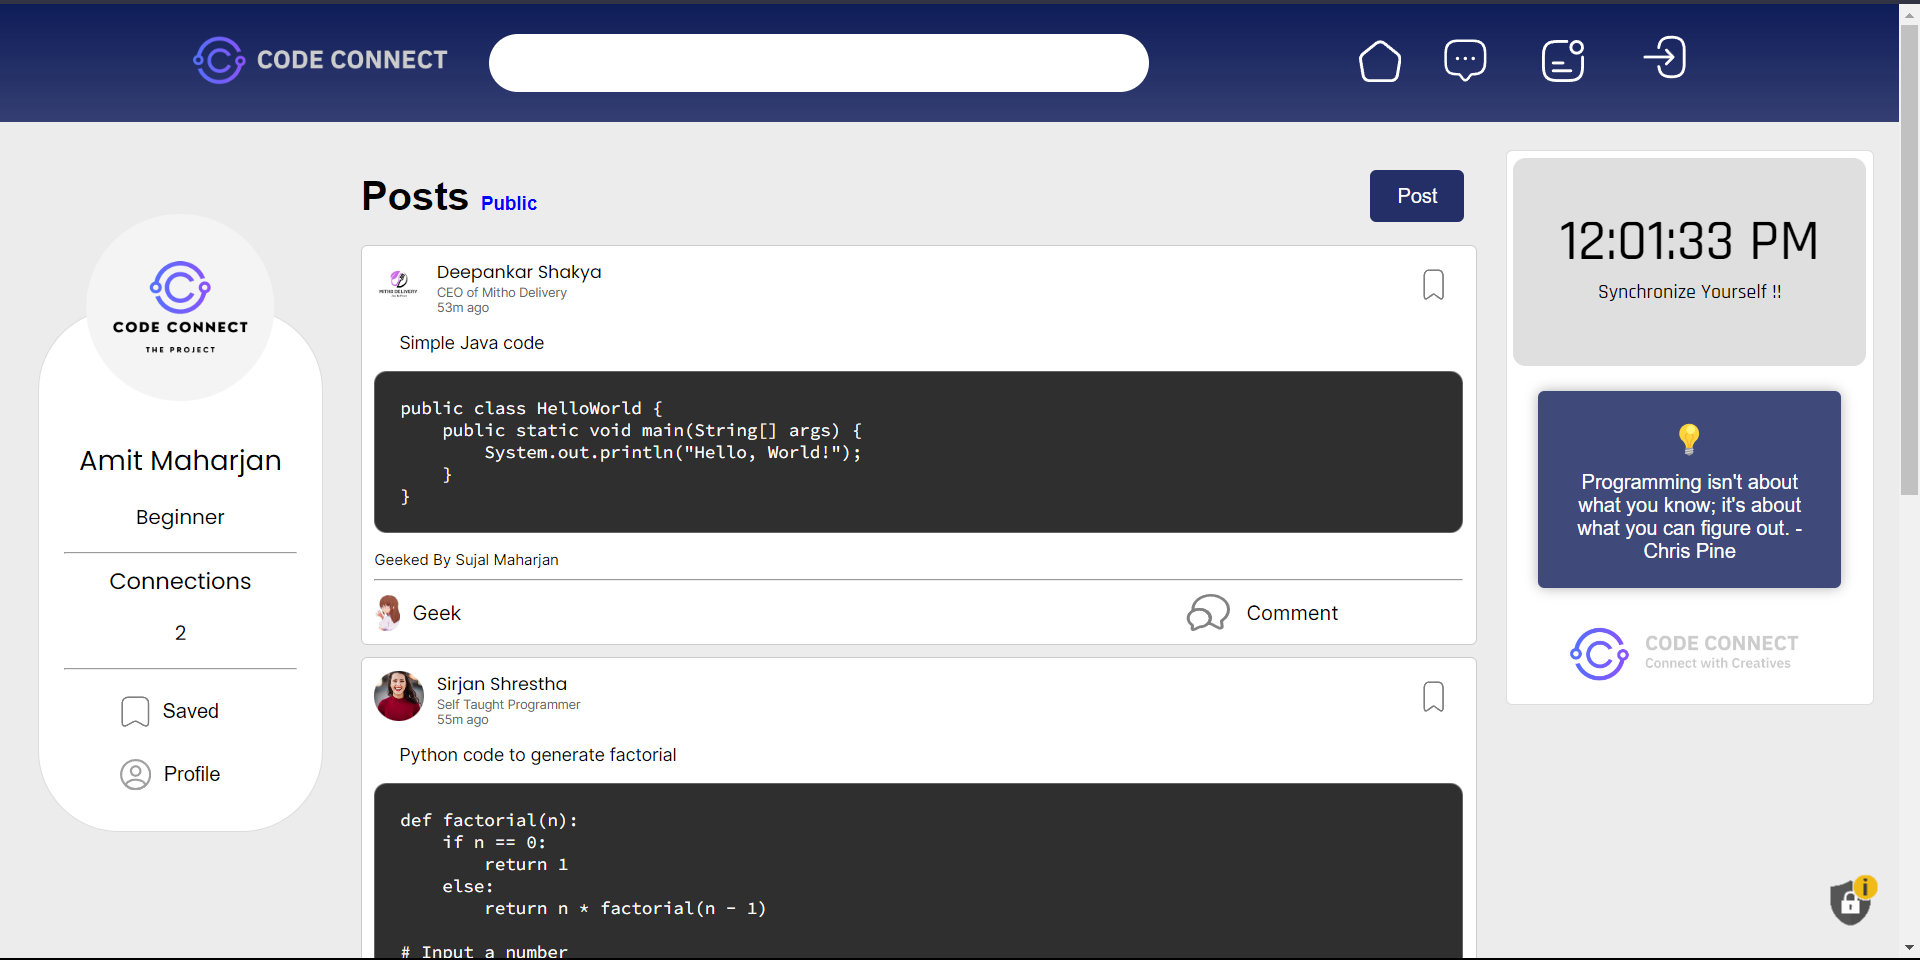
\includegraphics[width=1\textwidth]{Outcome-ss/homepage.png}
    \caption{Home Page.}
    \label{fig:Home Page}
\end{figure}

\textbf{Geek}
\\The image illustrates what happens when a user clicks on "geek." It's similar to how we use a "like" button to show we enjoy something. Pressing "geek" is like giving a thumbs up, showing that the user finds the content interesting or cool, much like using a "like" button.
\begin{figure}[ht]
    \centering
    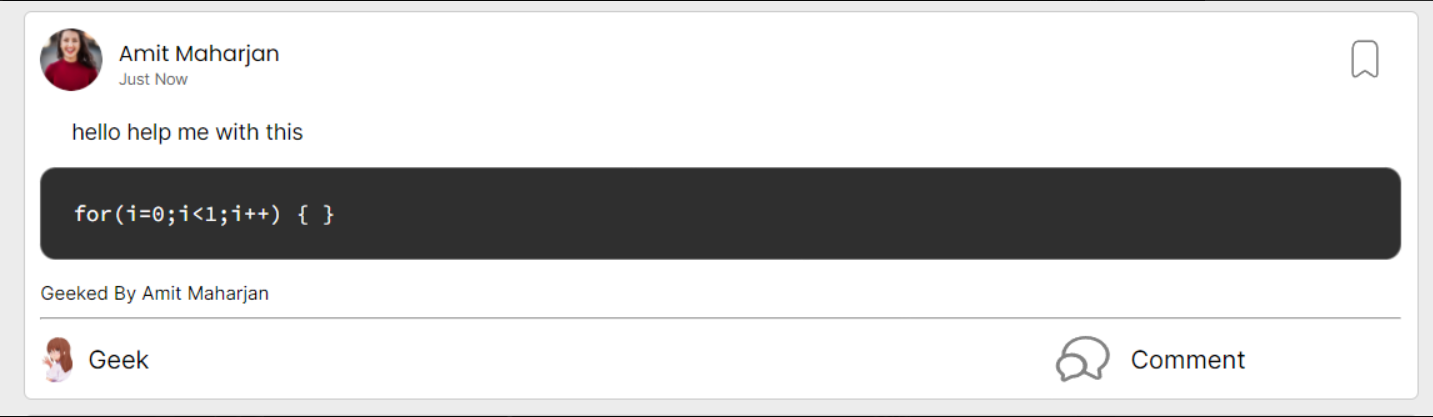
\includegraphics[width=0.5\textwidth]{Outcome-ss/geek.png}
    \caption{Geek.}
    \label{fig:Geek}
\end{figure}

\textbf{Un-Geek}
\\In the picture, you can see what happens when a user clicks "un-geek." It's like taking back a previous action, kind of like when you change your mind about liking something. Just as you can "unlike" by using a "dislike" button, "un-geek" lets you remove the interest or approval you showed earlier with the "geek" feature.
\begin{figure}[H]
    \centering
    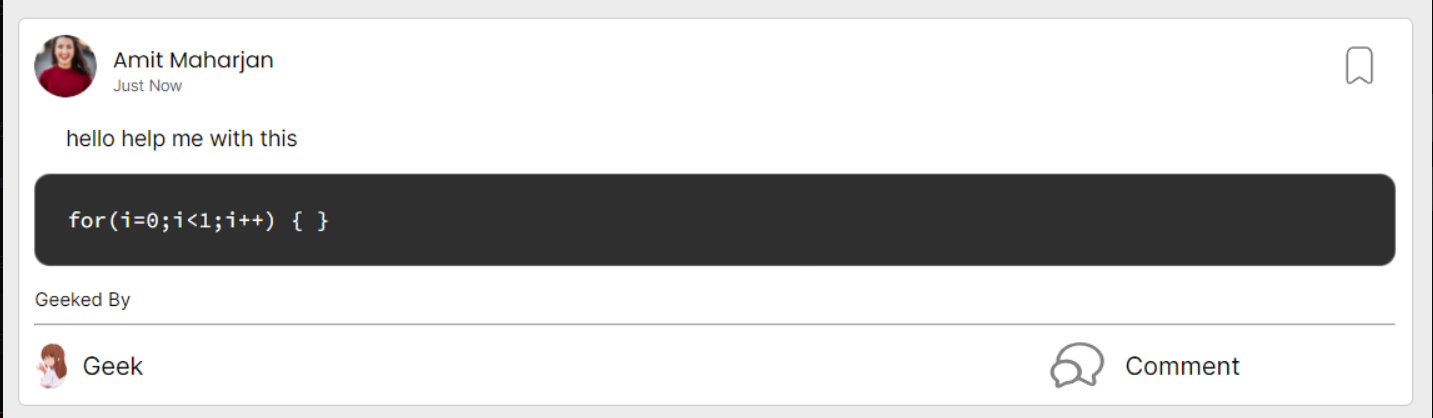
\includegraphics[width=0.5\textwidth]{Outcome-ss/ungeek.png}
    \caption{Un-Geek.}
    \label{fig:Un-Geek}
\end{figure}

\textbf{Profile}
\\The image displayed portrays the user profile within Code Connect. This profile presents a snapshot of the user's presence on the platform, offering insights into their activities, interests, and possibly their expertise. By showcasing key information, the profile facilitates connections and understanding among users, fostering a sense of community and collaboration within the Code Connect ecosystem.
\begin{figure}[ht]
    \centering
    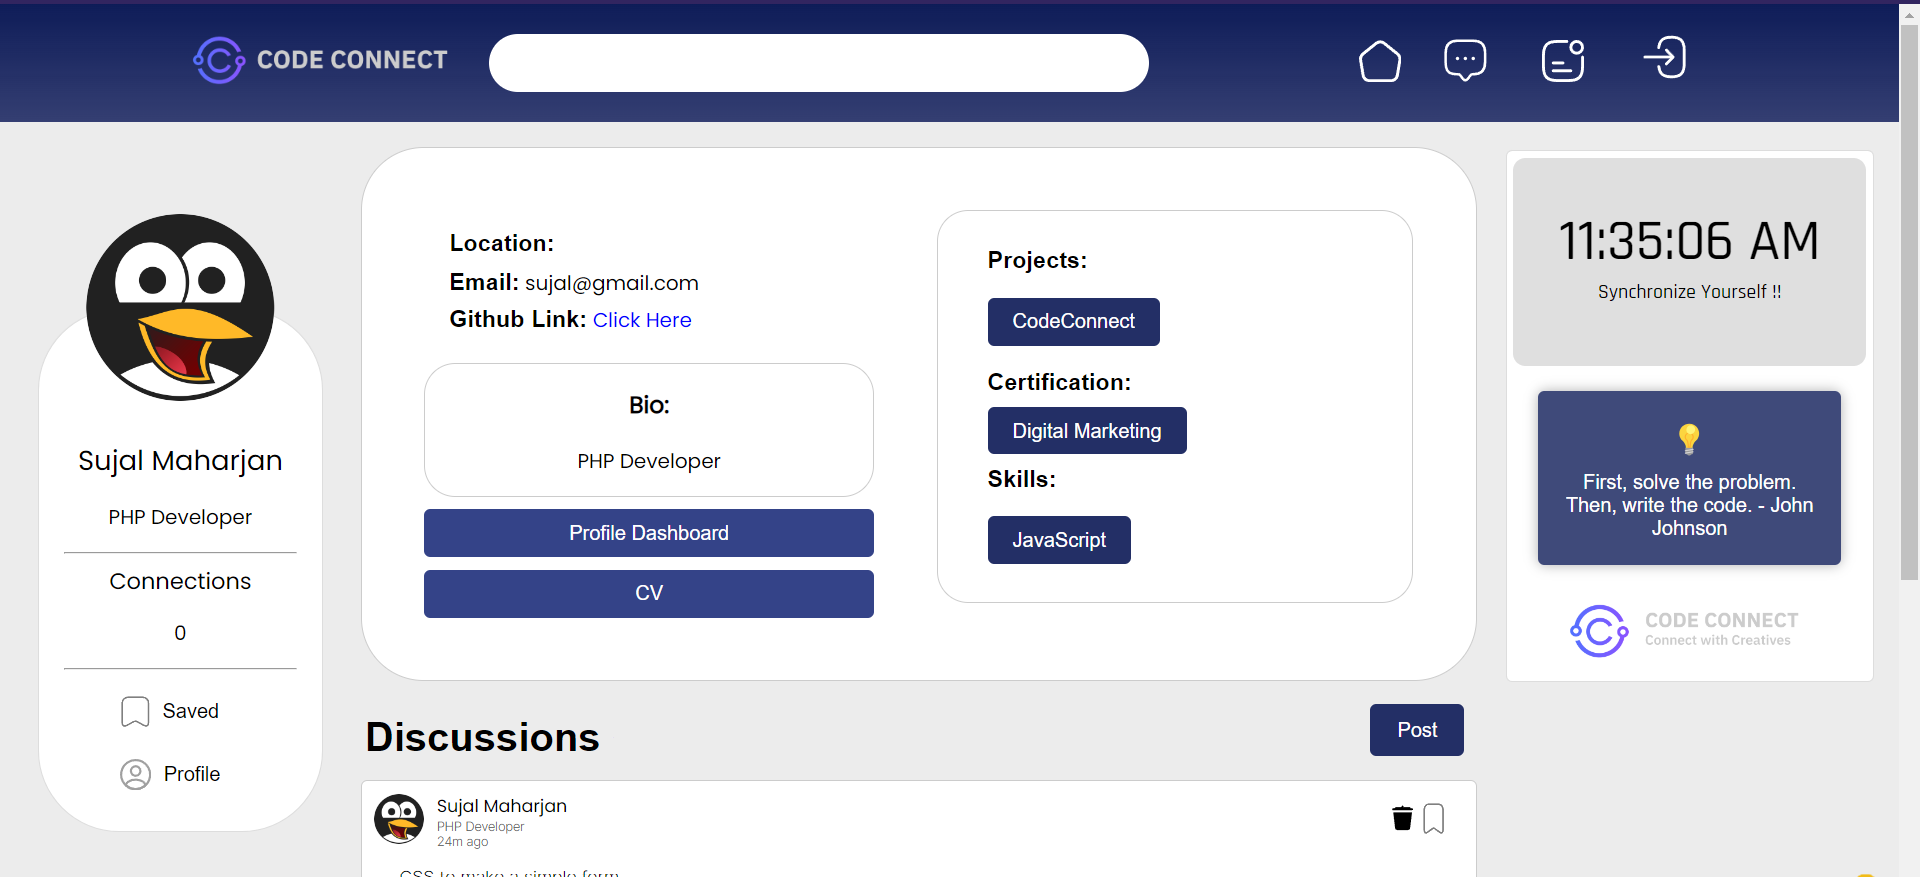
\includegraphics[width=1\textwidth]{Outcome-ss/self-profile.png}
    \caption{Profile.}
    \label{fig:Profile}
\end{figure}
\newpage
\textbf{Messanger}
\\In the picture, you can see the messaging part of Code Connect. It's like a chat where users can talk in real-time. This helps users easily share information, talk about projects, and ask for help within the Code Connect community. This messaging feature makes it simple for users to connect, share ideas, and work together on coding stuff.
\begin{figure}[ht]
    \centering
    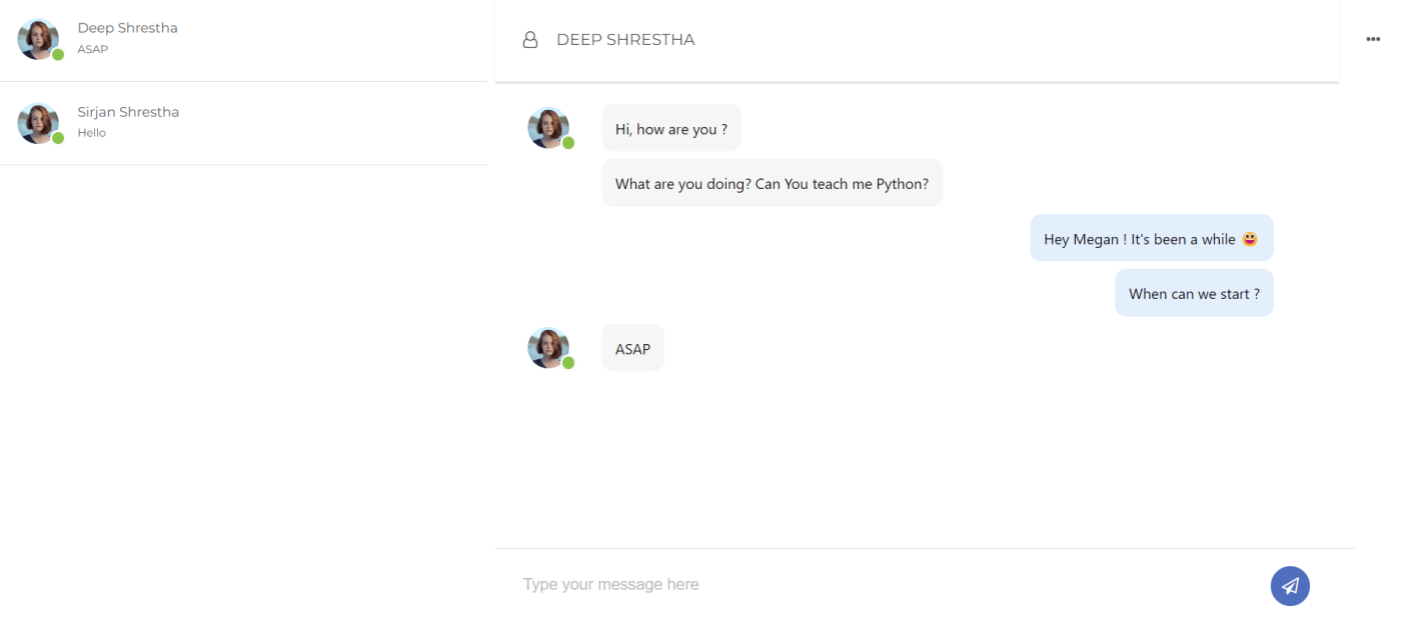
\includegraphics[width=1\textwidth]{Outcome-ss/messanger.png}
    \caption{Messenger.}
    \label{fig:Messenger}
\end{figure}

\textbf{Search}
\\"Code Connect" features an efficient search function where users can enter partial user names. As they type, the system dynamically suggests relevant user names that start with the typed letters. These suggestions appear in real-time below the search bar, aiding users in quickly finding and connecting with others. The process enhances user experience by providing instant, tailored recommendations based on the input, streamlining the connection process within the application.
\begin{figure}[ht]
    \centering
    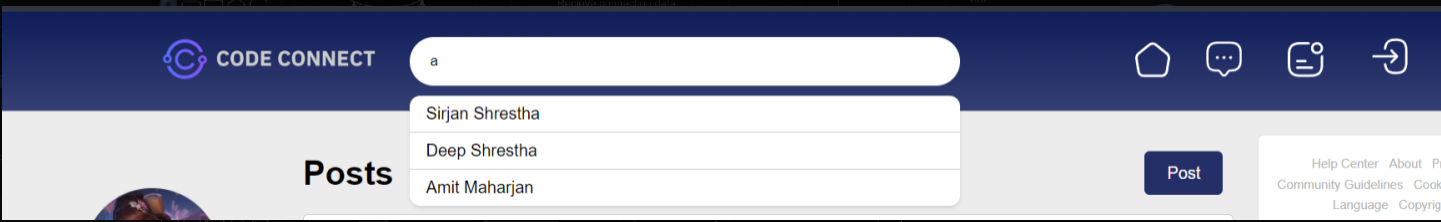
\includegraphics[width=0.5\textwidth]{Outcome-ss/search.png}
    \caption{Search.}
    \label{fig:Search}
\end{figure}

\textbf{Notification}
\\The image displayed below showcases the notification feature of Code Connect. This tool is designed to keep users informed about important updates and activities. Notifications ensure that users stay in the loop about significant interactions or changes within the platform. By providing these alerts, the notification system enhances user engagement and helps users effectively stay connected and engaged within the Code Connect community.
\begin{figure}[ht]
    \centering
    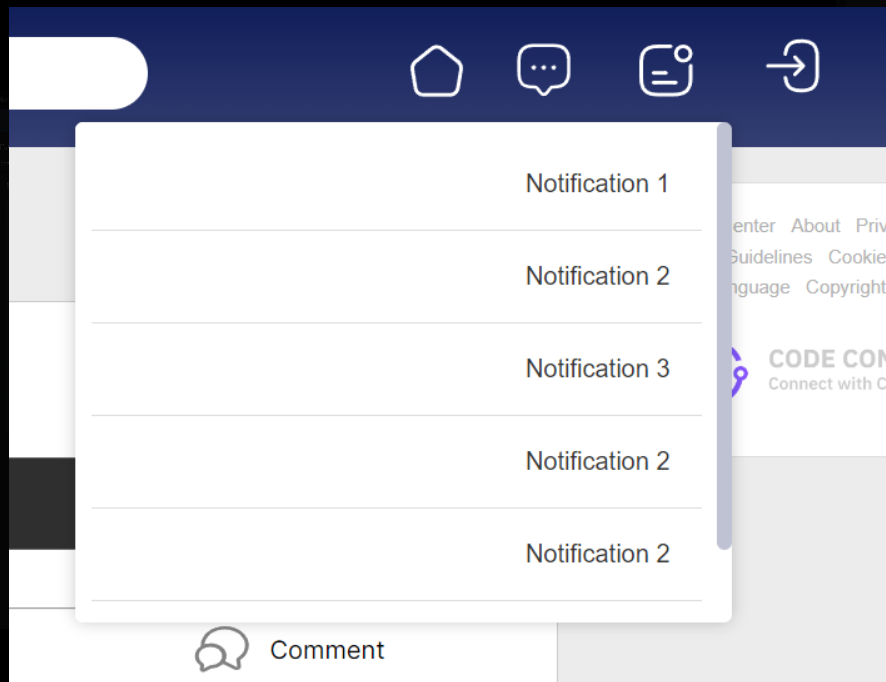
\includegraphics[width=0.5\textwidth]{Outcome-ss/notification.png}
    \caption{Notification.}
    \label{fig:Notification}
\end{figure}

\textbf{Post}
\\In the picture, you can see how you can make posts in Code Connect. It's like writing a message where you can share text and pieces of code. This helps you start conversations, show your coding work, and get advice from other users. It's a way to work together and learn from each other in Code Connect.
\begin{figure}[ht]
    \centering
    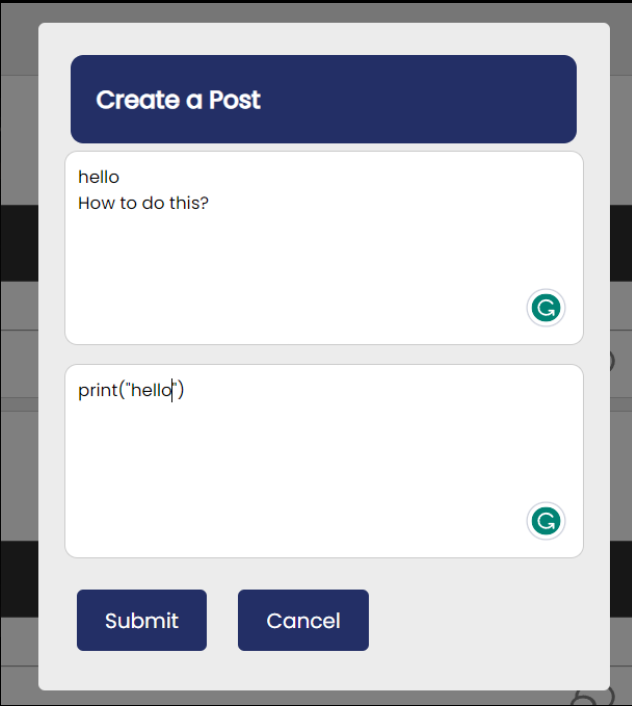
\includegraphics[width=0.5\textwidth]{Outcome-ss/post.png}
    \caption{Post.}
    \label{fig:Post}
\end{figure}

\textbf{Profile of other Users}
\\In the image below, you can see the profile section of other users. This section provides insights into their details, interests, and activities within the platform. By exploring these profiles, users can learn more about each other, their skills, and their contributions, fostering connections and collaboration within the community.
\begin{figure}[ht]
    \centering
    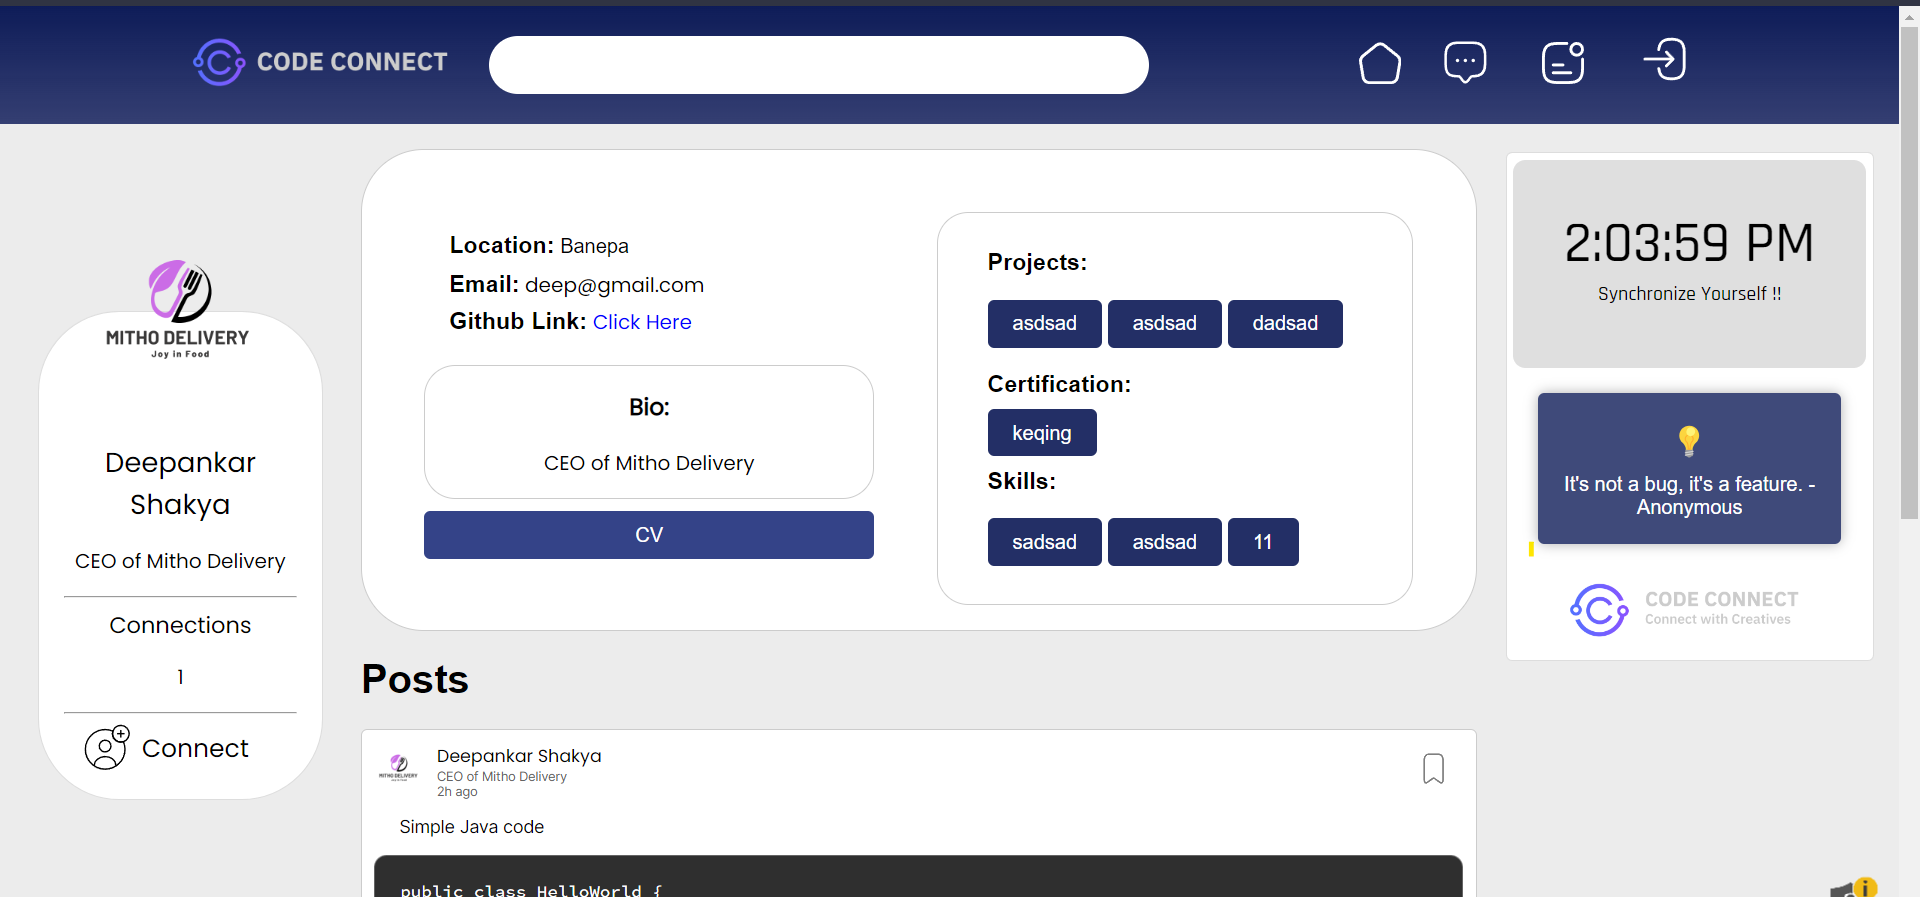
\includegraphics[width=1\textwidth]{Outcome-ss/other-user-profile.png}
    \caption{Profile of other Users.}
    \label{fig:Profile of other Users}
\end{figure}
\newpage
\textbf{Send Connection Request}
\\Sending a connection request is like asking someone if they want to be your friend on the platform. It's a way to show that you're interested in being connected and sharing things with them. If they accept, you can interact more and collaborate within the platform.
\begin{figure}[ht]
    \centering
    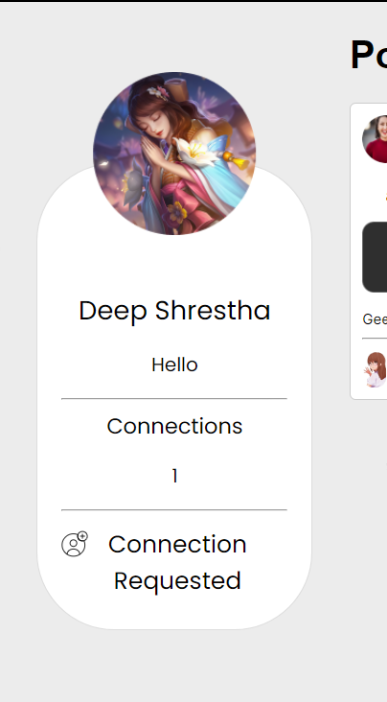
\includegraphics[height=0.3\textheight]{Outcome-ss/connection-request.png}
    \caption{Send Connection Request.}
    \label{fig:Send Connection Request}
\end{figure}

\textbf{Result after connection request is sent}
\\The image below gives you an idea of what it's like for another user when they receive a connection request. They'll see a notification that someone wants to connect with them. They can choose to accept the request and start connecting with the person who sent it. 
\begin{figure}[ht]
    \centering
    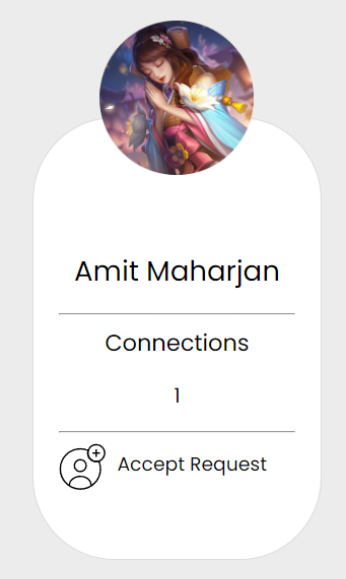
\includegraphics[height=0.3\textheight]{Outcome-ss/accept-request.png}
    \caption{Result after connection request is sent.}
    \label{fig:Result after connection request is sent}
\end{figure}
\newpage
\textbf{Connection Request Accepted}
\\If the request is accepted, you'll see a "connected" sign, showing you're now friends. The person who sent the request will be added to your list of friends. This makes it easy to find and talk to each other, so you can work together and share stuff within the platform.
\begin{figure}[ht]
    \centering
    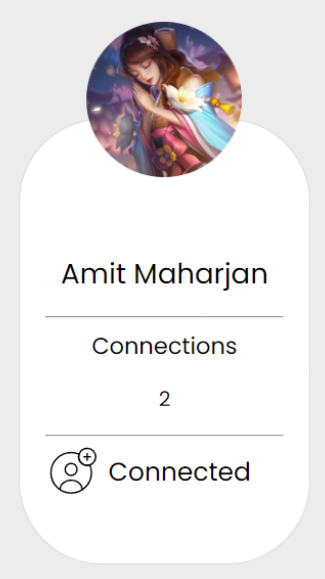
\includegraphics[height=0.3\textheight]{Outcome-ss/result-after-accepting.png}
    \caption{Connection Request Accepted.}
    \label{fig:Connection Request Accepted}
\end{figure}

\section{Conclusion}
Code Connect is a social networking web application designed specifically for creative it professionals. It should transform the way developers connect, collaborate, and learn from each other. The platform provides a range of features that allow creative it professionals to network, share knowledge, and enhance their skills. Code Connect also fosters a vibrant and inclusive resume and portfolio management system.
